\subsubsection{10.12.14}

\begin{enumerate}
	\item Время начала и окончания собрания:
	17:30 - 21:00
	\item Цели собрания:
	\begin{enumerate}
	  \item Установить стальные перекладины на робота.
	  
	  \item Обсудить идеи по решению проблемы с опрокидыванием ковша.
	  
    \end{enumerate}
	\item Проделанная работа:
	\begin{enumerate}
	  \item На робота была установлена только одна перекладина.
	  
	  \begin{figure}[H]
	  	\begin{minipage}[h]{0.2\linewidth}
	  		\center  
	  	\end{minipage}
	  	\begin{minipage}[h]{0.6\linewidth}
	  		\center{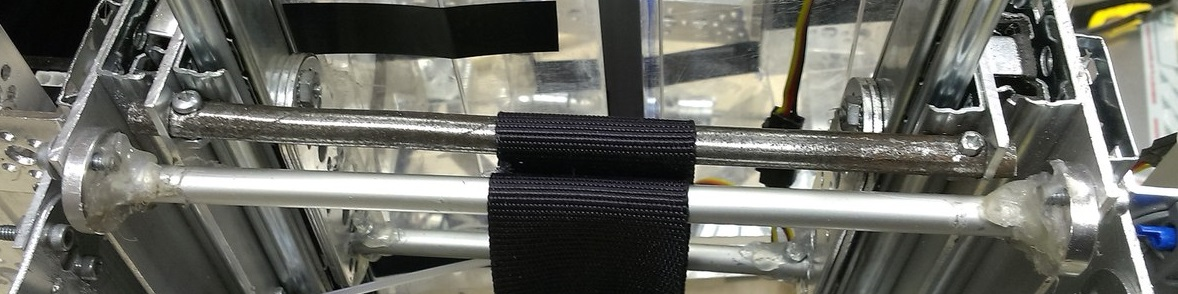
\includegraphics[scale=0.3]{days/10.12.14/images/01}}
	  		\caption{Стальная перекладина}
	  	\end{minipage}
	  \end{figure}
	  
	  \item Для решения проблемы с опрокидыванием ковша было решено установить на верхнюю часть ковша механизм, который будет до старта робота фиксировать пружину, которая будет раздвигать плечо с грузами, уравновешивающее ковш с мячами (таким образом будет решена проблема с ограничением робота по высоте до начала игры). Кроме того, было решено использовать для опрокидывания ковша не один, а два сервопривода.
	  
	 % \begin{figure}[H]
	 % 	\begin{minipage}[h]{0.2\linewidth}
	 % 		\center  
	 % 	\end{minipage}
	 % 	\begin{minipage}[h]{0.6\linewidth}
	 % 		\center{
\includegraphics[scale=0.3]{days/10.12.14/images/02}}
	 % 		\caption{Идея механизма}
	 % 	\end{minipage}
	 % \end{figure}
      
    \end{enumerate}
    
	\item Итоги собрания: 
	\begin{enumerate}
	  \item Стальная перекладина установлена.
	  
	  \item Разработана идея установки раздвижного противовеса на ковш для того, чтобы его было легче опрокидывать.
	  
	  \item Было решено добавить сервопривод на механизм опрокидывания ковша.
	  
    \end{enumerate}
    
	\item Задачи для последующих собраний:
	\begin{enumerate}
	  \item Завершить установку стальных перекладин на подъемник.
	  
	  \item Создать механизм противовеса для ковша.
	  
	  \item Добавить сервопривод на механизм опрокидывания ковша.
	  
    \end{enumerate}     
\end{enumerate}
\fillpage